% Author: Kevin Zhu, Risheek Pingili
% Email: kevonz31@berkeley.edu

\qns{Basic Function Interpolation}

  Given a set of points $\{ (\frac{\pi}{4} ,\frac{\sqrt{2}}{2}),(\frac{3\pi}{4} ,\frac{\sqrt{2}}{2}),(\frac{5\pi}{4},\frac{-\sqrt{2}}{2}), (\frac{7\pi}{4} ,\frac{\sqrt{2}}{2})\}$ interpolate and graph the function using:

\begin{enumerate}
	\qitem Linear Interpolation
	\sol{ Since we have 4 data points to use, each at the interval (or $\delta$) of $\frac{\pi}{2}$, we can get our $\phi(x)$ for each point according to the equation
	\begin{align*}
	\phi(x) = \begin{cases}
	                1-\frac{1-\mid x \mid}{\frac{\pi}{2}} & |x| \leq \delta \\
	      			0 & \text{else} \\
	   		    \end{cases}
	\end{align*}
	Plugging in x for each point we get:
	\begin{align*}
	\phi (x) = \begin{cases}
	                1-\frac{1-\mid x-\frac{\pi}{4} \mid}{\frac{\pi}{2}} & |x|\leq\delta \\
	      			0 & \text{else} \\
	   		    \end{cases}
	\end{align*}
	\begin{equation*}
	\phi(x) = \begin{cases}
	                1-\frac{1-\mid x-\frac{3\pi}{4} \mid}{\frac{\pi}2} & |x|\leq\delta \\
	      			0 & \text{else} \\
	   		    \end{cases}
	\end{equation*}
	\begin{equation*}
	\phi(x) = \begin{cases}
	                1-\frac{\mid x- \frac{5\pi}{4} \mid}{\frac{\pi}2} & |x|\leq\delta \\
	      			0 & \text{else} \\
	   		    \end{cases}
	\end{equation*}
	\begin{equation*}
	\phi(x) = \begin{cases}
	                1-\frac{\mid x-\frac{7\pi}{4} \mid}{\frac{\pi}2} & |x|\leq\delta \\
	      			0 & \text{else} \\
	   		    \end{cases}
	\end{equation*}
	We then scale each $\phi(x)$ by its respective y component and plot all of them on the graph.
		Perhaps an easier way to think about this graphically is to draw each (x , y) point on a graph and draw the linear function (a v pointing towards the x axis from the given point) for each point that you’ve drawn.
		\begin{center}
    		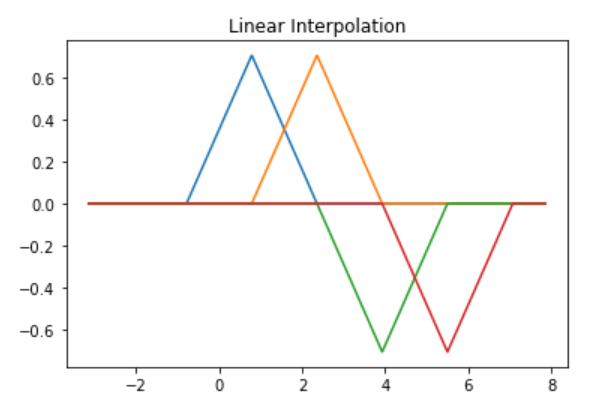
\includegraphics[width=4in]{\bank/interpolation/figures/linear_interpolation.png}
	  	\end{center}
		Next, we would add all of the graphs together so that it satisfies our equation where $y = \sum_i{y_i \cdot \phi(x_i)}$ for each given point i. After scaling and adding all of our graphs together, here’s what it looks like:
		\begin{center}
    		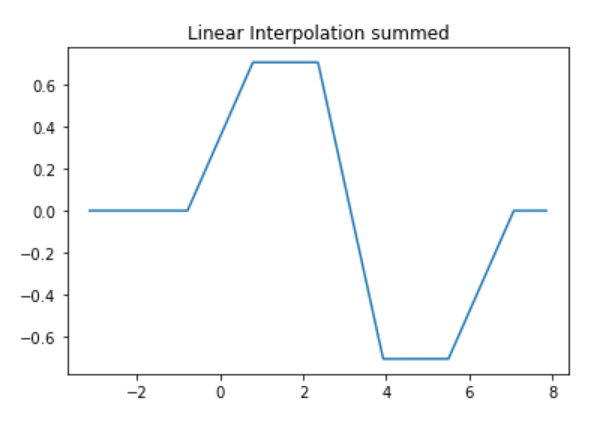
\includegraphics[width=4in]{\bank/interpolation/figures/linear_interpolation_summed.png}
	  	\end{center}
	}


  \vspace{10cm}
	\qitem Zero-hold interpolation
	\sol{ Zero-hold involves treating eah point as a fixed value for its entire duration. The $\phi$ funciton is
		\begin{equation*}
		\phi(x) = \begin{cases}
	                1 \hspace{1cm} \, x\in [0,\delta) \\
	      			0 \hspace{1cm} \, \text{else} \\
	   		    \end{cases}
	\end{equation*}
		Essentially, we’re now drawing straight line segment for every point in that we are given, and then we scale according to the y coordinate. \\
		Here's what that looks like for our points after adding and scaling (you'll noittce that the functions overlap):
		\begin{center}
    		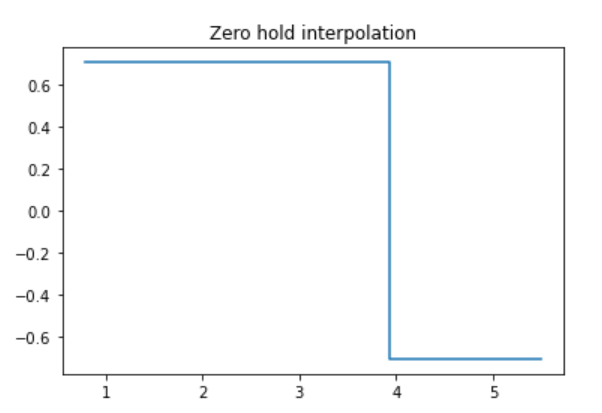
\includegraphics[width=4in]{\bank/interpolation/figures/zero_hold_interpolation.png}
	  	\end{center}
		}

  \vspace{10cm}
	\qitem Sinc interpolation
	\sol{Once again, we separate each point by a phi function, which in this case is the sinc function:
		\begin{equation*}
		\phi(x) = \begin{cases}
	                \frac{sin(\pi \cdot x)}{\ pi \cdot x} \hspace{1cm} \, x\neq 0 \\
	      			1 \hspace{3cm} \, x=0 \\
	   		    \end{cases}
		\end{equation*}
		Here's what the sinc function looks like:
		\begin{center}
    		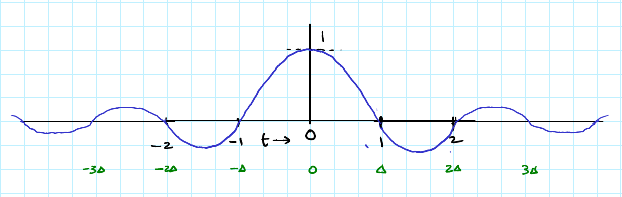
\includegraphics[width=4in]{\bank/interpolation/figures/sinc.png}
	  	\end{center}
		Our $\phi(x)$ function is $sinc(\frac{x}{\delta} )$, which is a sinc function at each point of x. \\
		Here’s what each scaled functions look like layered on top:
		\begin{center}
    		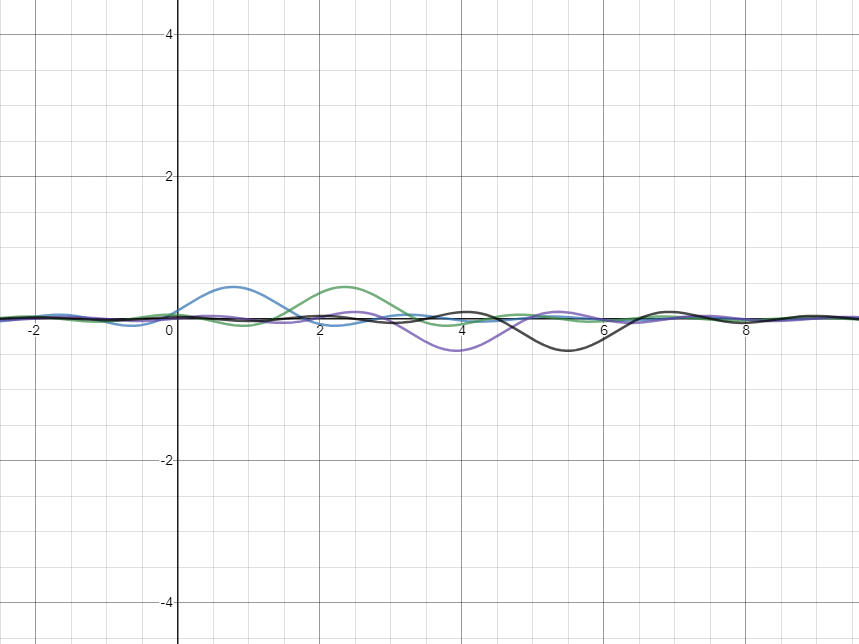
\includegraphics[width=4in]{\bank/interpolation/figures/sinc_interpolate.png}
	  	\end{center}
		And added together:
		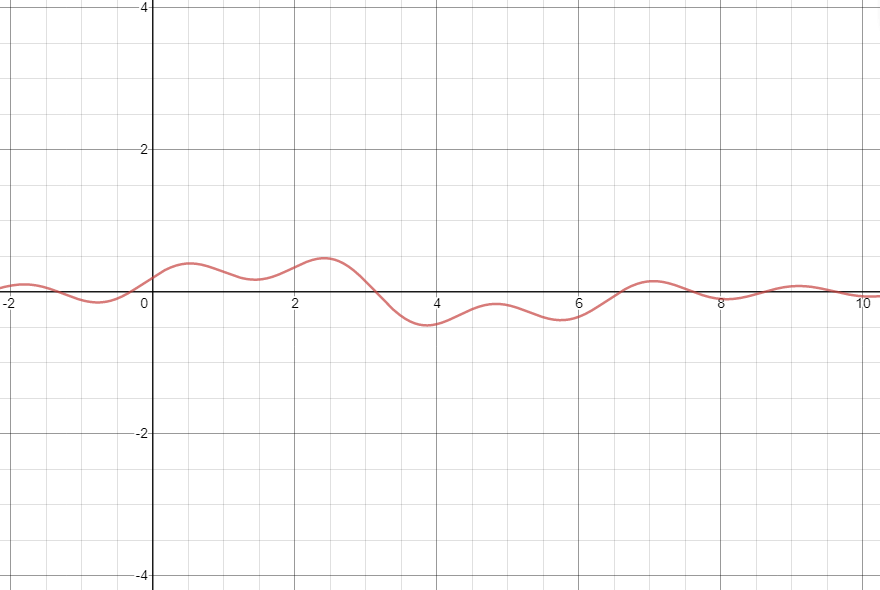
\includegraphics[width=4in]{\bank/interpolation/figures/sinc_interpolation.png}
	}

  \vspace{10cm}


	\qitem Now, we'll run sinc interpolation using different points: $\{ (\frac{\pi}{4} ,\frac{\sqrt{2}}{2}),(\frac{7\pi}{4} ,\frac{\sqrt{2}}{2}),(\frac{11\pi}{4},\frac{-\sqrt{2}}{2}), (\frac{13\pi}{4} ,\frac{\sqrt{2}}{2})\}$
	Is this similar to the last function?

		\meta{Allude to Nyquist theorem}

		\sol{ There's a lot less symmetry in this function, and it also doesn't capture the same waveform: it's negative and positive in different areas.
    The function that we've sampled all of our points from is the sine function.
    How do parts a to c compared to the sinc function? This last interpolation seems to be quite different.
    Is this from the asymmetric sampling, or the varying frequency?
\begin{center}
    		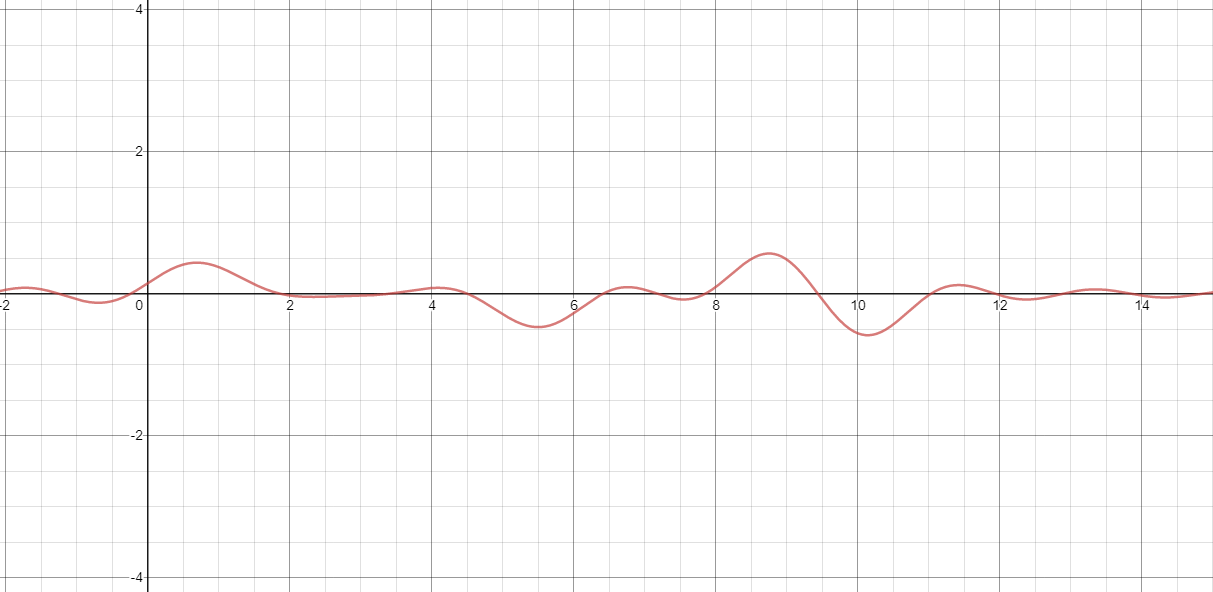
\includegraphics[width=4in]{\bank/interpolation/figures/sinc_interpolation2.png}
	  	\end{center}}
\end{enumerate}
